\section{Model 1}

The results displayed in this section are for the
activation energy for the fall off reaction in the ozone
mechanism. The percentage of ozone is taken as 40, 46, 53, 75 and 100
percent according to the experimental data
available~\cite{Streng}. In the
figure~\ref{subfig-1:Raw Chain} and figure~\ref{subfig-2:Histogram} ,  we display results for sample size 1e7 and surrogate
of 1000 points. We show the raw samples generated by MCMC and plot
 the histogram for parameter $E_3$. In the figure~\ref{fig-2:conv_sample} , for
constant surrogate size, the number of samples are changed from 1e5 to
1e7 and convergence is observed. The plot is done for surrogate size of 1000 and raw chain size of $1e5$, $5e5$ , $1e6$, $5e6$ and $1e7$ is taken. In the figure~\ref{fig-3:conv_surrogate},
convergence study is done for surrogates with differing number of
interpolation points. As we increase the number of points in the surrogate, results should be close for different surrogate sizes. The plot is done for surrogate size of 100, 500 and 1000. In this analysis, raw sample chain size is $1e7$. For different starting points of MCMC chain, the MAP point of the resulting pdf does not change. The surrogates for individual
concentrations are constructed using linear interpolation
function. The initial guess for the MAP point is calculated using
Nelder Mead optimization technique. 

\bigskip

In the
figure~\ref{subfig-1:mean_1} and figure~\ref{subfig-2:auto_11},  mean and correlation plots are shown for
the samples of the parameter. The mean plot shows the initial instability due to sum in period of MCMC and after that it remains constant. It shows us that we should be using at least more than these number of samples for our analysis. The figure~\ref{subfig-2:final_e3} shows the posterior of the parameter $E_3$ with the following parameters of the distribution- Mean:  28.3, Std. Dev.:  0.78, Skewness:  0.066 and Kurtosis:  0.035.

\bigskip

 It is necessary to ensure that the samples of the parameter which we are drawing are fitting the flamespeed values of the experiment. In the figure~\ref{subfig-1:40_1}, figure~\ref{subfig-2:46_1}, figure~\ref{subfig-3:53_1}, figure~\ref{subfig-4:75_1}, and figure~\ref{subfig-5:100_1},   we calculate the flamespeed for all the parameters drawn using the surrogate generated before for 40$\%$, 46$\%$, 53$\%$, 75$\%$, and 100 $\%$ respectively. We have taken $1e7$ sample size and calculated flamespeed for all the concentrations of ozone mentioned. We have a good fit to the data overall.



%\subsection{Convergence Study: Number of Samples }

% In this section, we see the convergence of the probability distribution as we increase the raw chain sample size. The plot is done for surrogate size of 1000. In this analysis, raw chain size of $1e5$, $5e5$ , $1e6$, $5e6$ and $1e7$ is taken.



%\subsection{Convergence Study: Surrogate }

 %In this section, we see the convergence of the surrogate. As we increase the number of points in the surrogate, results should be close for different surrogate sizes. The plot is done for surrogate size of 100, 500 and 1000. In this analysis, raw sample chain size is $1e7$.



%\subsection{Flamespeed data fit}

 %It is necessary to ensure that the samples of the parameter which we are drawing are fitting the flamespeed values of the experiment. In this section, we calculate the flamespeed for all the parameters drawn using the surrogate generated before. We have taken $1e7$ sample size and calculated flamespeed for different concentrations of ozone.

 


%\subsection{Mean and Autocorrelation Plots}

% In this section, we show the mean of the samples and autocorrelation plots . The mean plot shows the initial instability due to sum in period of MCMC and after that it remains constant. It shows us that we should be using at least more than these number of samples for our analysis. The last figure shows the histogram and the various parameters of the distribution are Mean:  28.3, Std. Dev.:  0.78, Skewness:  0.066 and Kurtosis:  0.035.






\begin{figure}[H]
\subfloat[MCMC raw chain of samples \label{subfig-1:Raw Chain}]{%
     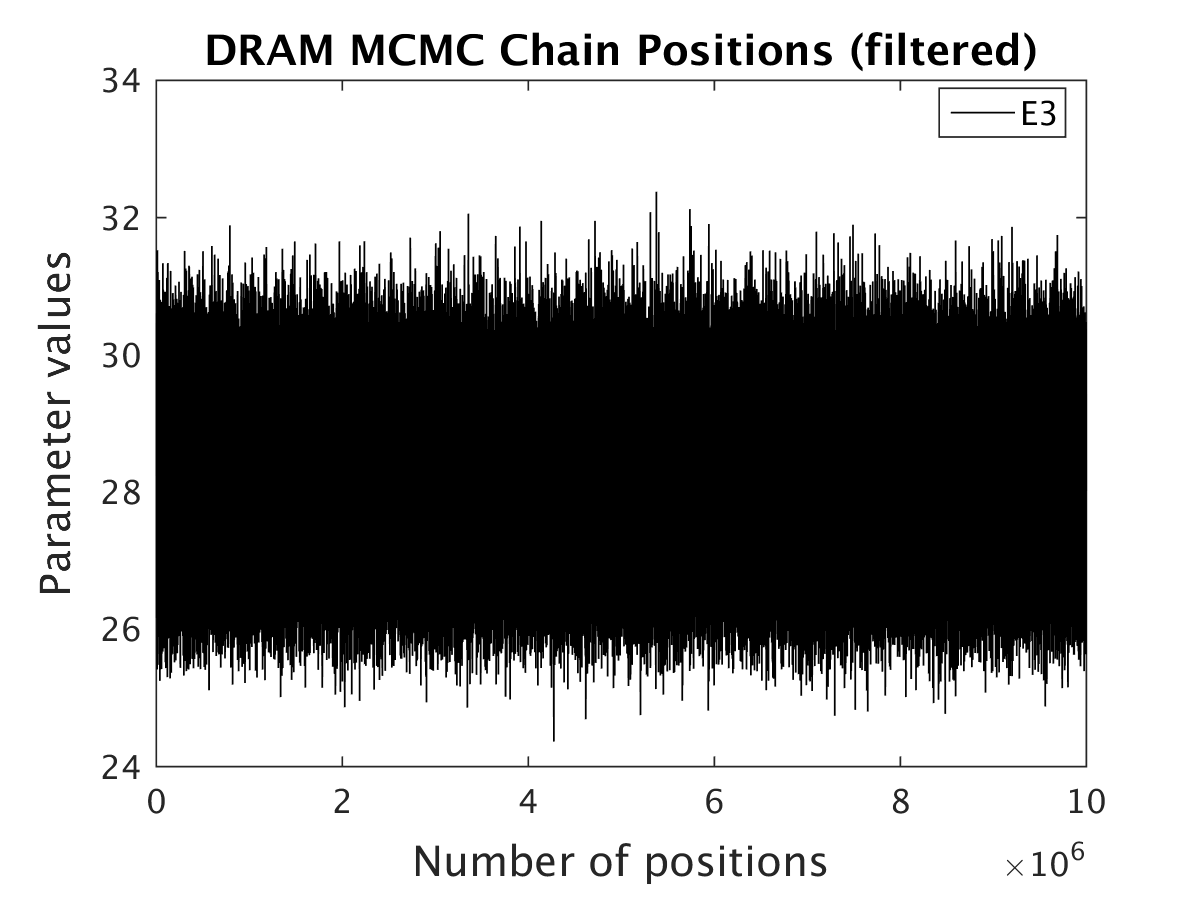
\includegraphics[scale=0.45]{model_1/simple_ip_chain_pos_filt}
    }
\subfloat[Histogram\label{subfig-2:Histogram}]{%
     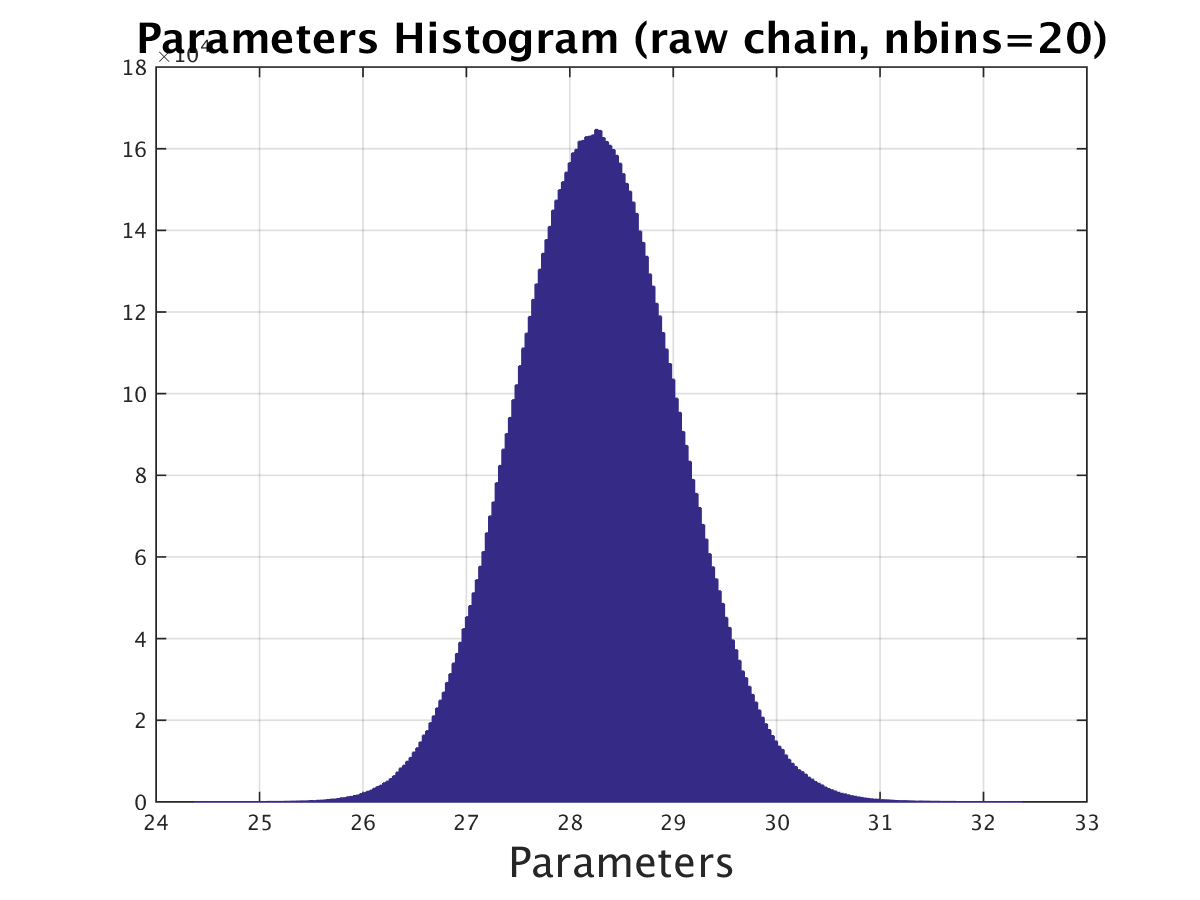
\includegraphics[scale=0.47]{model_1/simple_ip_hist_raw}
    }
\caption{MCMC raw chain and histogram}
    \end{figure}
%
  \begin{figure}[H]
  \ContinuedFloat
  \centering
\subfloat[KDE \label{subfig-4:KDE_1}]{
        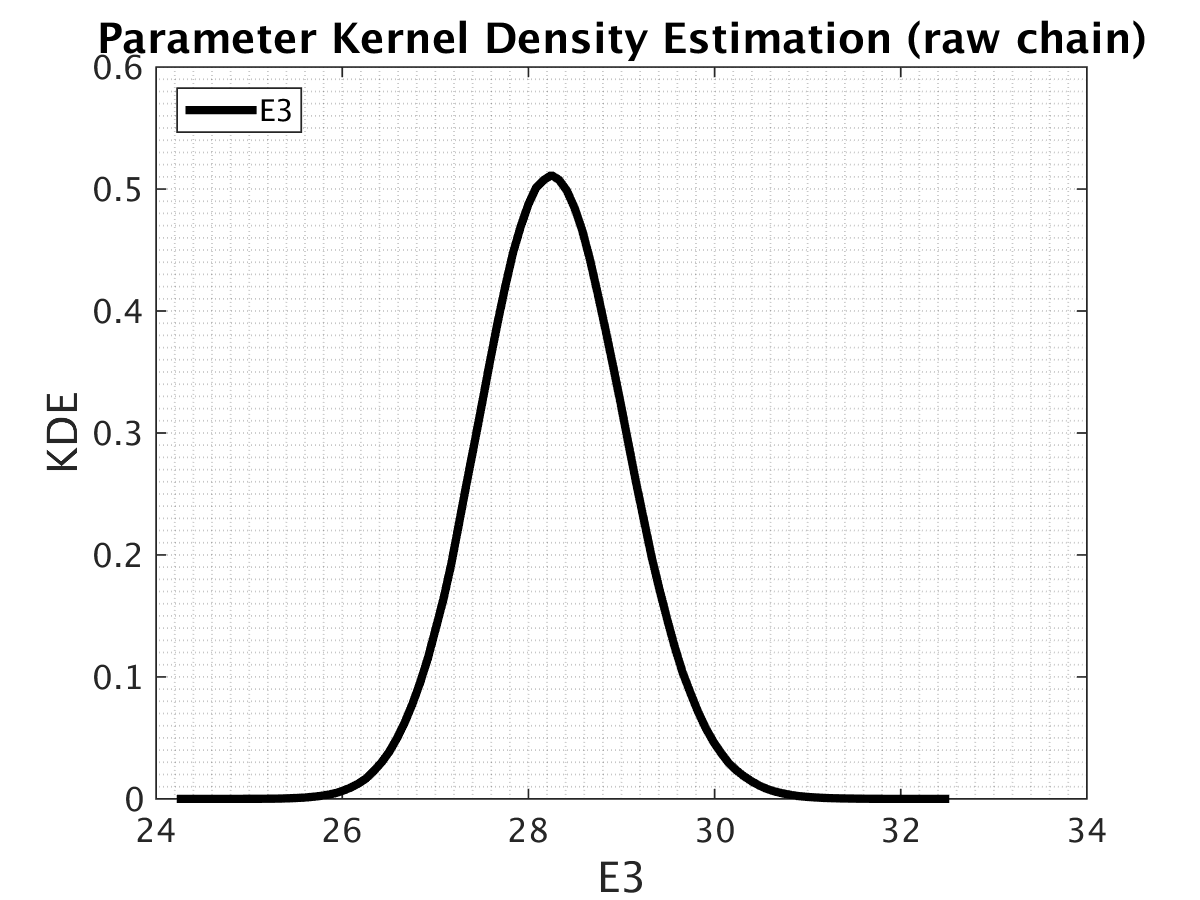
\includegraphics[scale=0.7]{model_1/simple_ip_kde_raw}
            }
\caption{ Parameter  kernel density estimation for $E_3$}
\end{figure}


\begin{figure}[H]
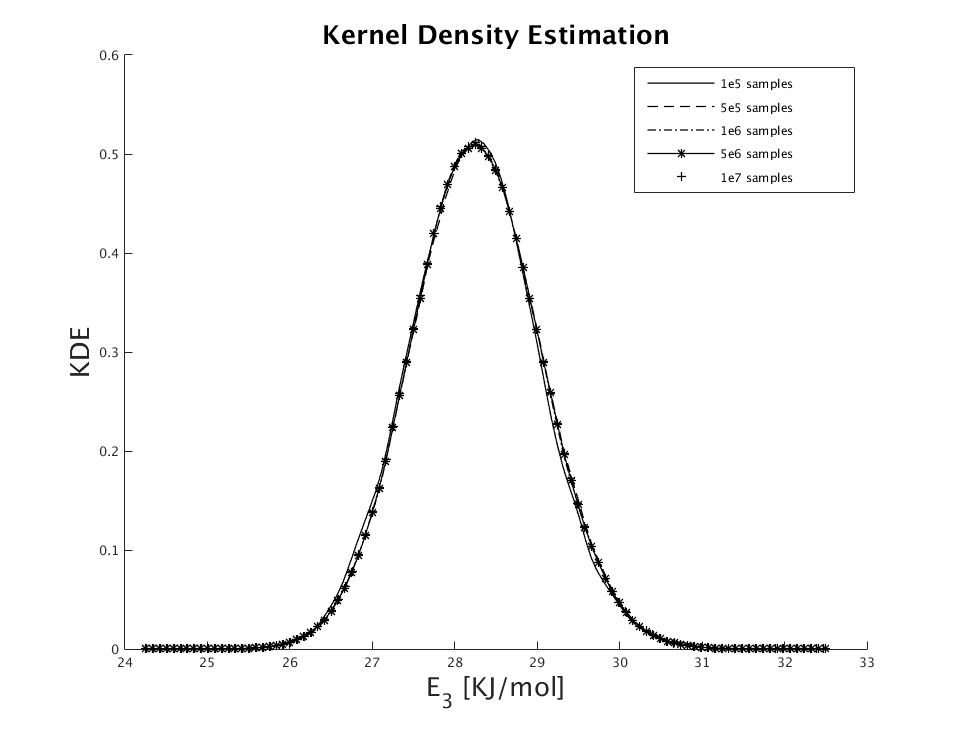
\includegraphics[scale = 0.5]{model_1/sample_conv}
    \caption{Convergence for surrogate size 1000}
    \label{fig-2:conv_sample}
\end{figure}



\begin{figure}[H]
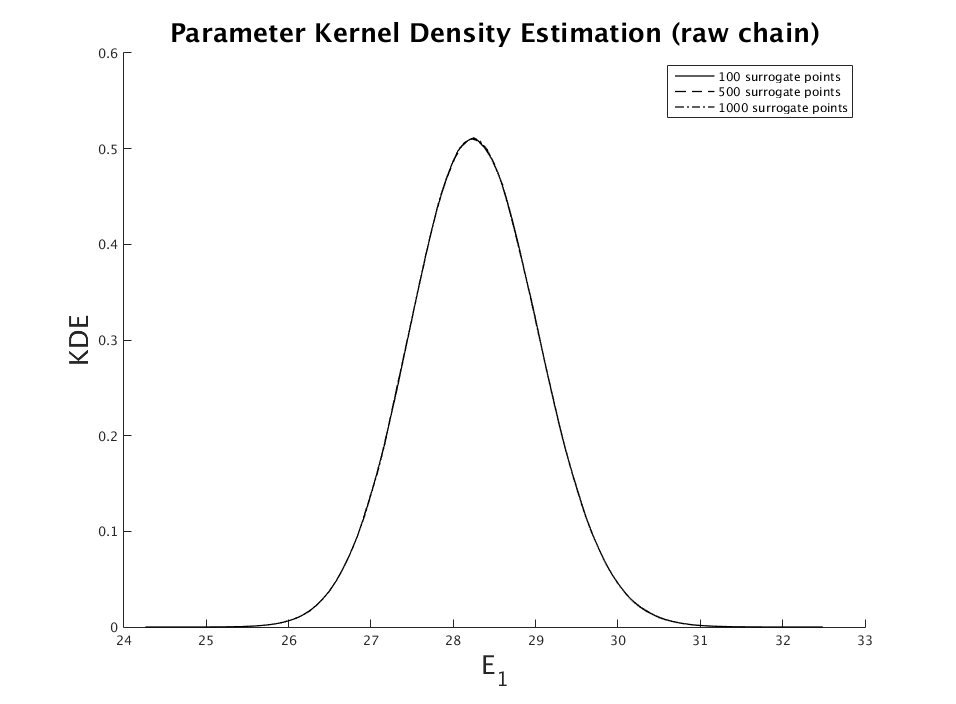
\includegraphics[scale=0.5]{model_1/conv_surrogate}
    \caption{Convergence for surrogate size 100, 500 and 1000}
    \label{fig-3:conv_surrogate}
\end{figure}


\begin{figure}[H]
   \subfloat[ Flame speed for 40 \% ozone \label{subfig-1:40_1}]{
        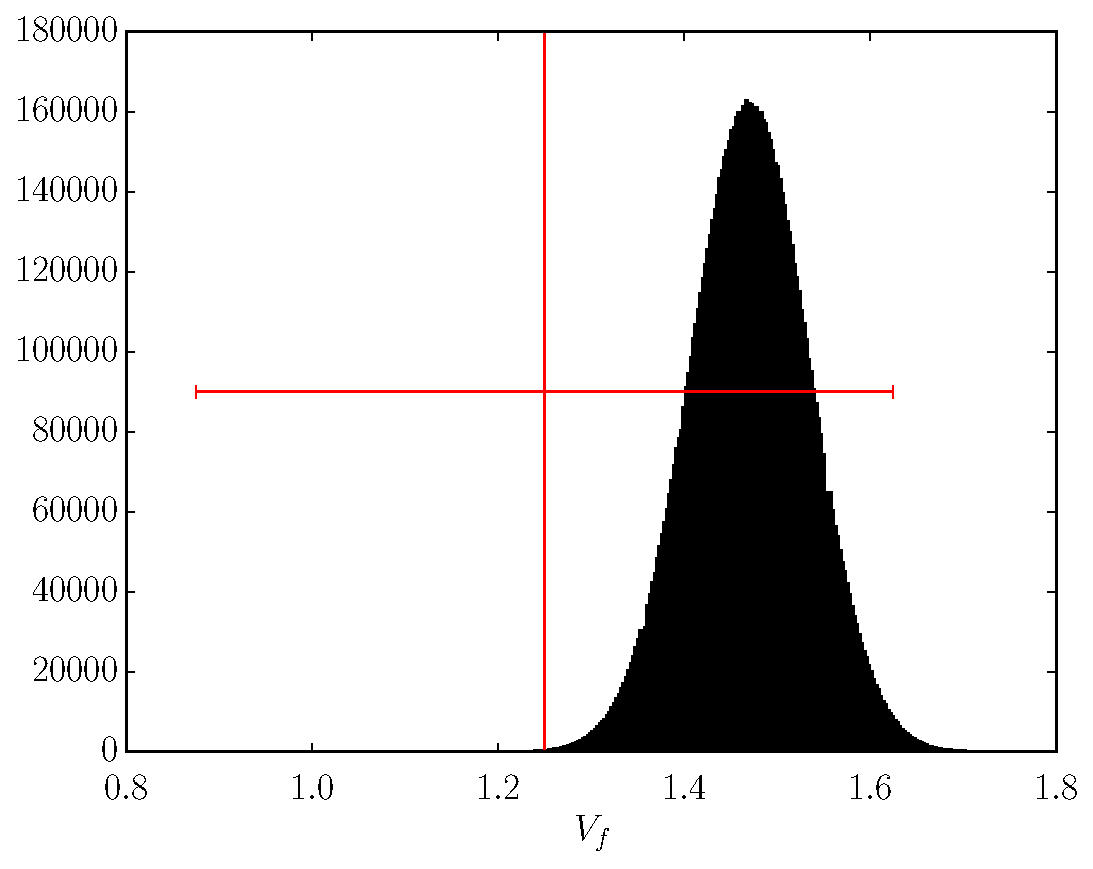
\includegraphics[scale=0.45]{model_1/flame_40.pdf}
       }
\subfloat[Flame speed for 46 \% ozone \label{subfig-2:46_1}]{
        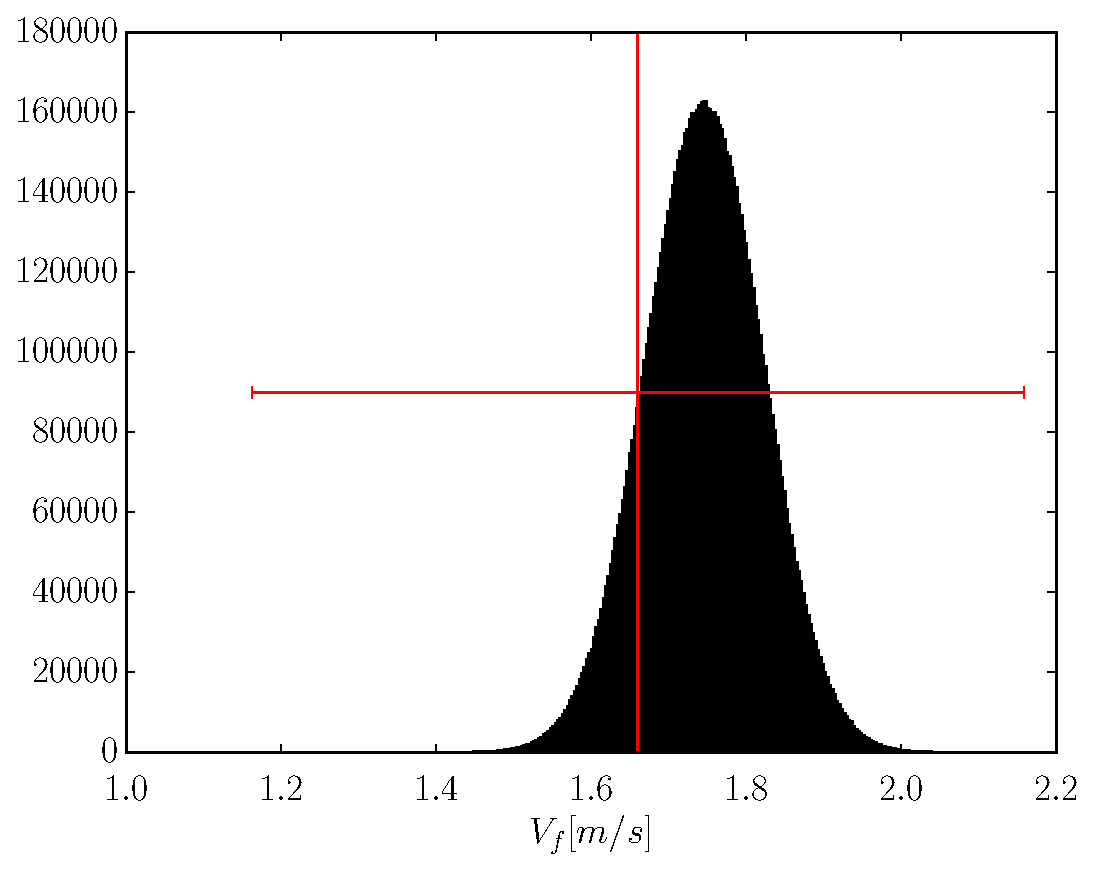
\includegraphics[scale=0.45]{model_1/flame_46.pdf}
            }
\end{figure}


 \begin{figure}[H]
  \ContinuedFloat
   \subfloat[ Flame speed for 53 \% ozone \label{subfig-3:53_1}]{
        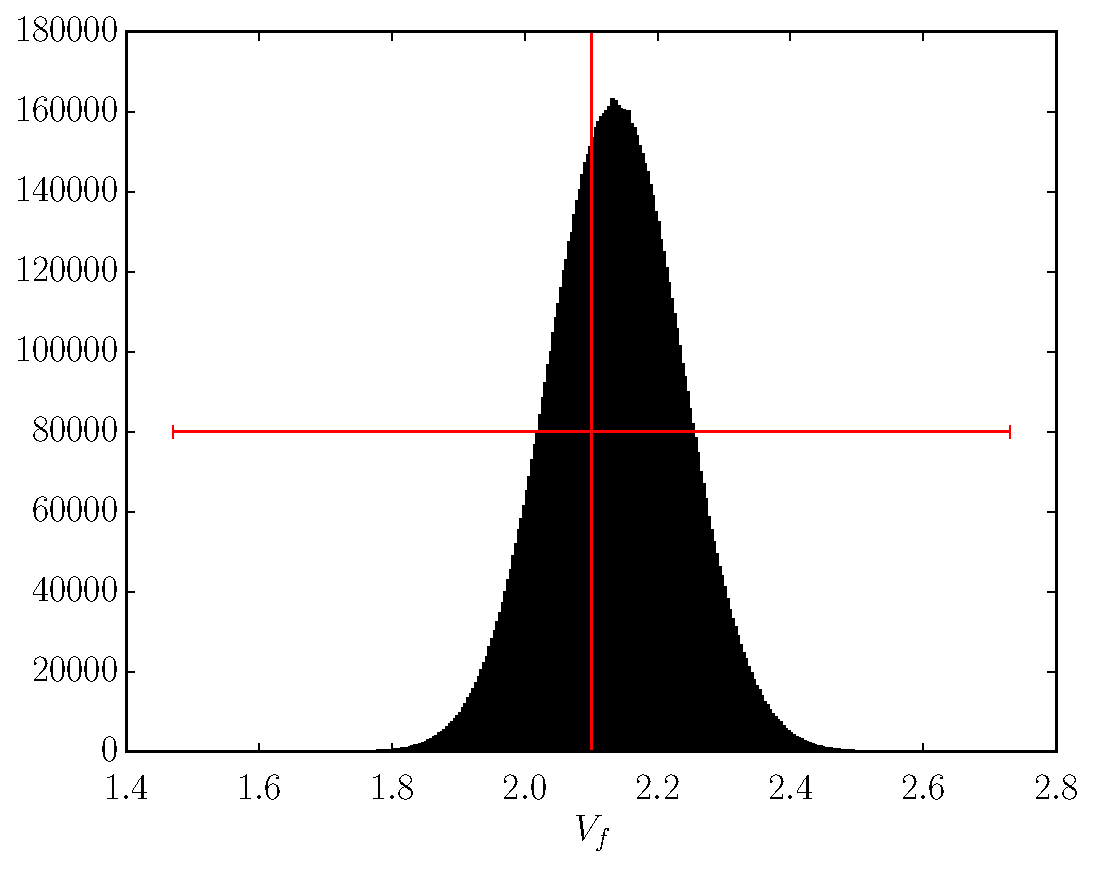
\includegraphics[scale=0.45]{model_1/flame_53.pdf}
       }
\subfloat[Flame speed for 75 \% ozone \label{subfig-4:75_1}]{
        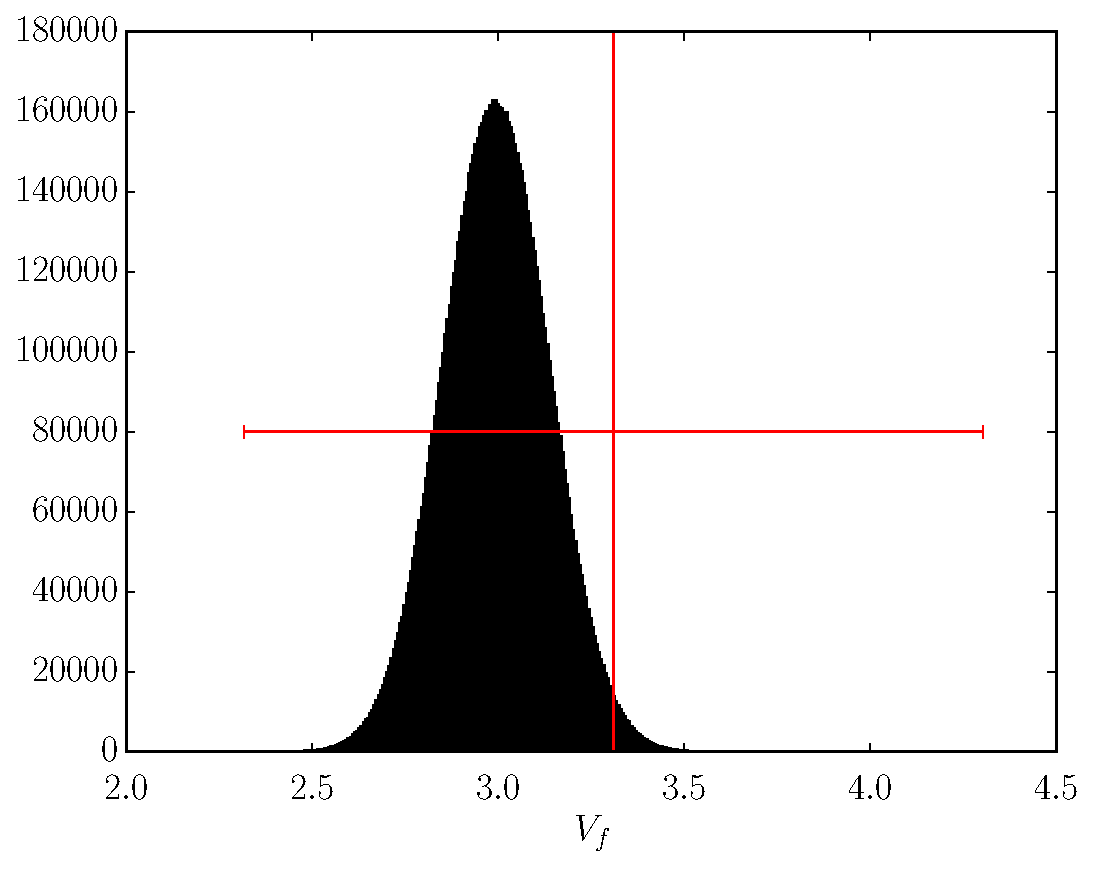
\includegraphics[scale=0.45]{model_1/flame_75.pdf}
            }
\end{figure}


 \begin{figure}[H]
  \ContinuedFloat
   \subfloat[ Flame speed for 100 \% ozone \label{subfig-5:100_1}]{
        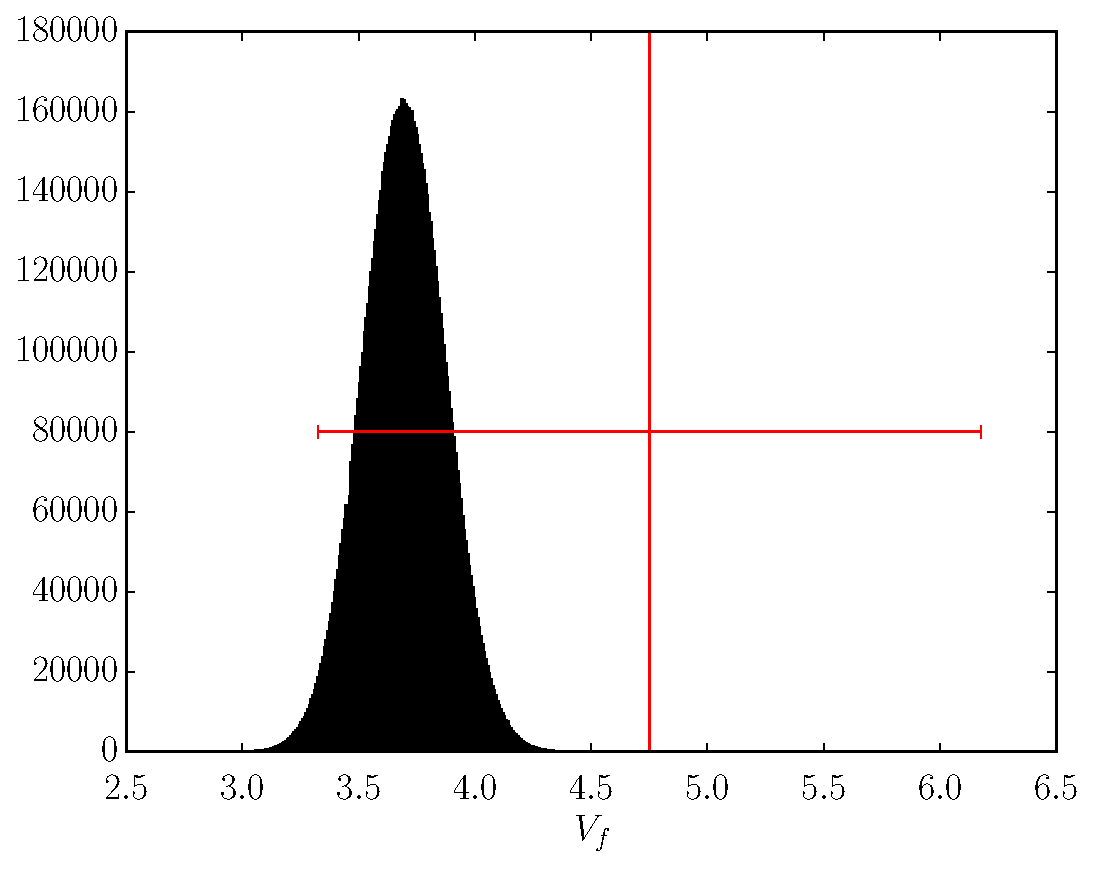
\includegraphics[scale=0.45]{model_1/flame_100.pdf}
       }
  \caption{Flamespeed Data Fit}
\end{figure}


 \begin{figure}[H]
  \ContinuedFloat
  \centering
   \subfloat[ Mean  \label{subfig-1:mean_1}]{
        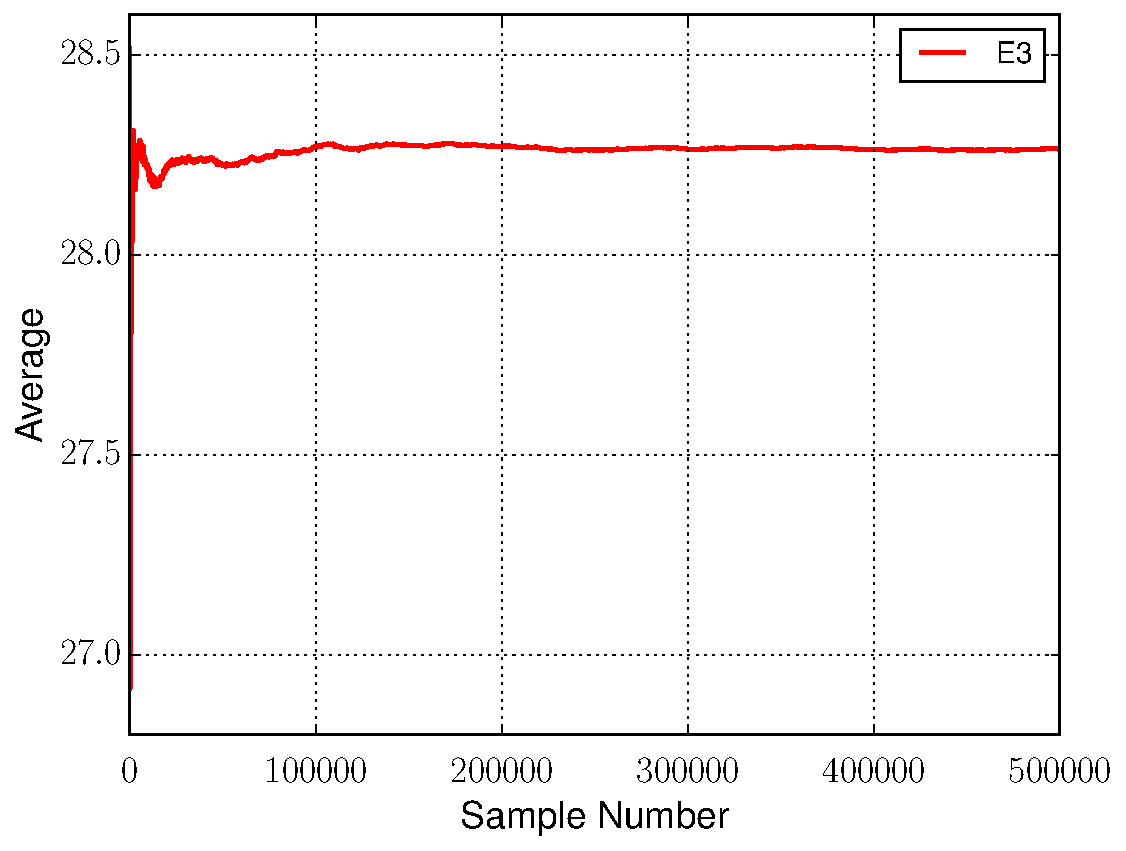
\includegraphics[scale=0.7]{model_1/M1_running_avg.pdf}
       }
     \quad
\subfloat[Autocorrelation  \label{subfig-2:auto_11}]{
        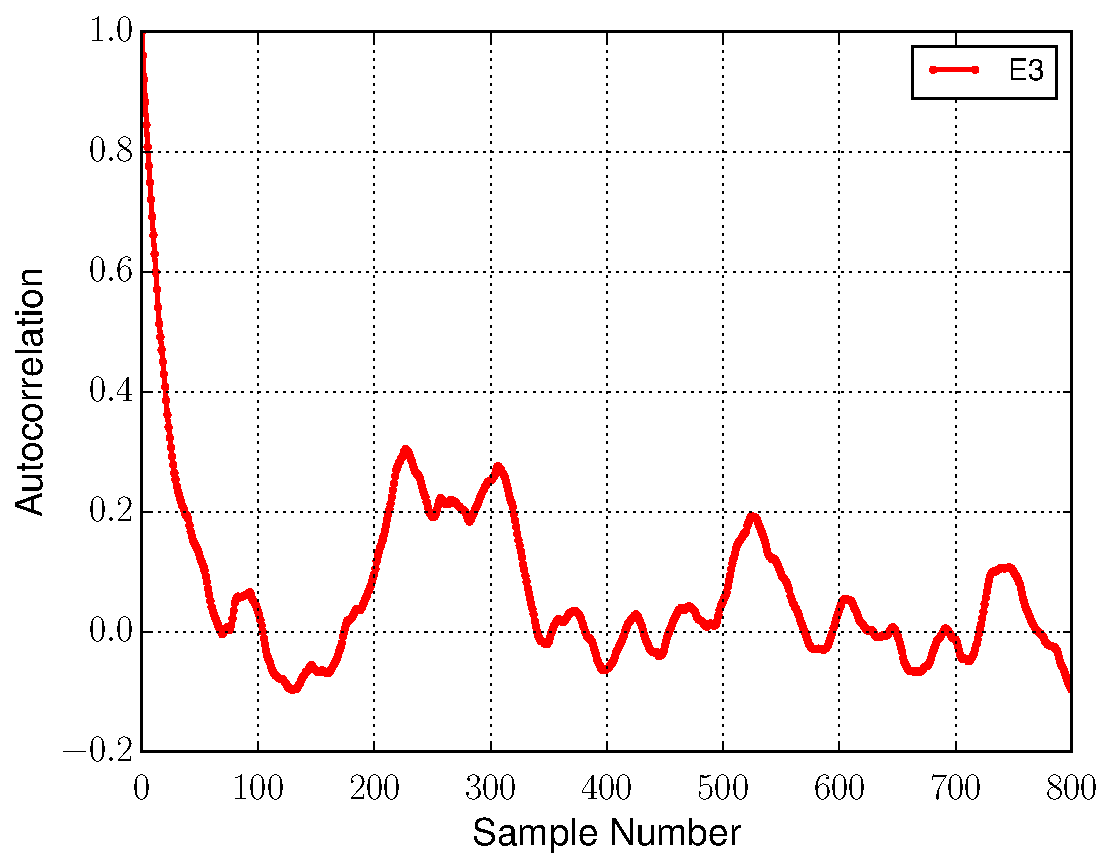
\includegraphics[scale=0.7]{model_1/M1_autocorr.pdf}
            }
            \caption{Mean and autocorrelation for sample size 1e7}
			\end{figure}
 \begin{figure}[H]
  \centering
\subfloat[ \label{subfig-2:final_e3}]{
        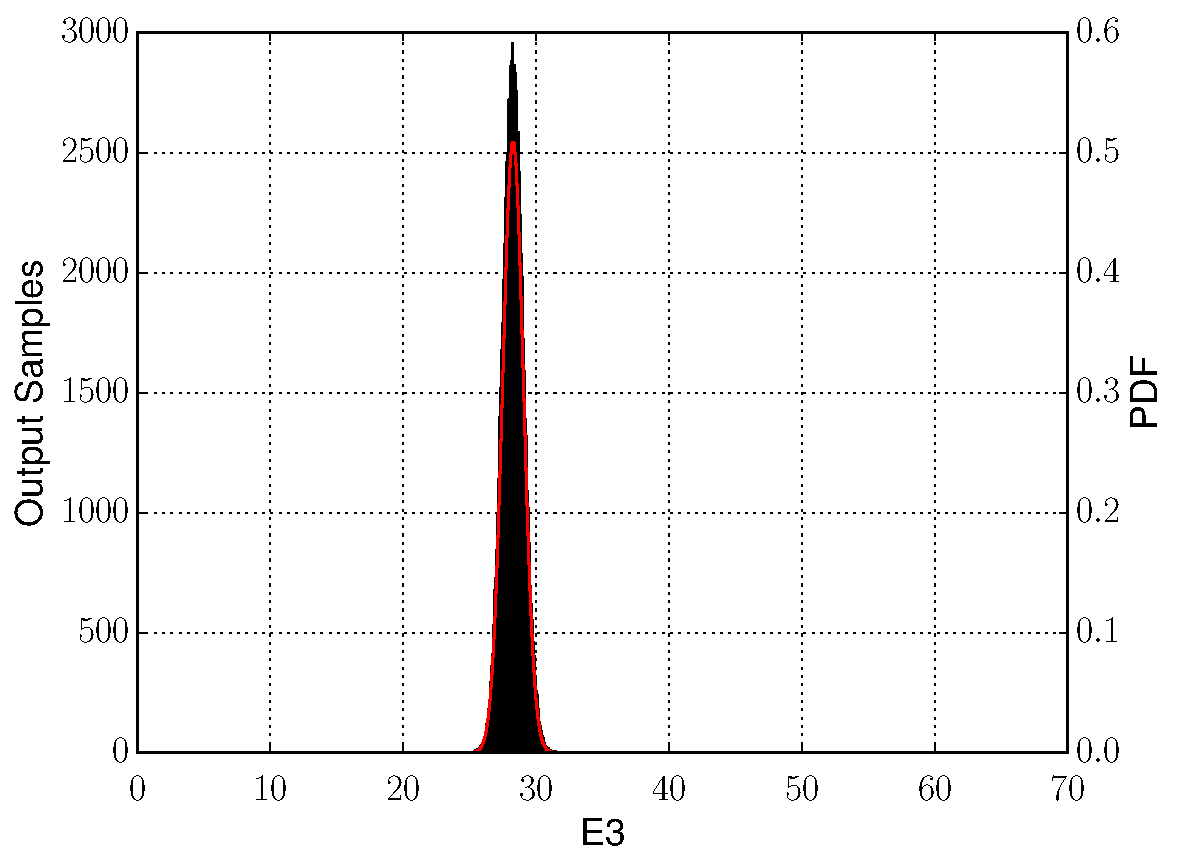
\includegraphics[scale=0.7]{model_1/E3.pdf}
            }
            \caption{$E_3$ posterior distribution}
\end{figure}


